\chapter{Анализ трёх аспектов современных стран по Викиданным: возраст стран, популярные формы правления и этнохоронимы}
\label{ch:country}

Эта глава посвящена исследованию стран на основе базы знаний международного проекта Викиданные. С помощью SPARQL-запросов, вычисляемых на объектах <<страна>> в Викиданных, получены: список всех ныне существующих стран, перечень стран, упорядоченных по дате создания, список этнохоронимов стран, пузырьковая диаграмма с формами правления стран и граф соседних стран. Кроме того, проанализирована полнота Викиданных по данной теме.
%%%%%%%%%%%%%%%%%%%%%%%%%%%%%%%%%%%%%%%%%%%%%%%%%%%%%%%
\section{Экземпляры}

Построим список всех стран на английском и русском языках (листинг ~\ref{lst:country}).

\begin{lstlisting}[ language=SPARQL, 
caption={\href{https://w.wiki/k6L}{Экземпляры объекта <<Страна>>}\protect\footnotemark},
label=lst:country, 
escapebegin=ку,escapeend=ку-ку>
]
#List of countries in English and Russian
SELECT ?country ?label_en ?label_ru
WHERE
{
		?country wdt:P31 wd:Q6256. # country
		?country rdfs:label ?label_en filter (lang(?label_en) = "en").
		?country rdfs:label ?label_ru filter (lang(?label_ru) = "ru").
}
\end{lstlisting}

\footnotetext{Получено 205 записей на 2017 год и 175 записей на 2020 год. Ссылка на SPARQL-запрос: \href{https://w.wiki/k6L}{https://w.wiki/k6L}}

Примерами наиболее полных и проработанных стран на Викиданных являются:  \wdqName{Соединённые Штаты Америки}{30}, \wdqName{Канада}{16}, \wdqName{Испания}{29}.

Почти пустыми и малоинформативными странами являются: \wdqName{Сахарская Арабская Демократическая Республика}{40362}, \wdqName{Приднестровская Молдавская Республика}{907112}, \wdqName{Косово}{1246}.

%%%%%%%%%%%%%%%%%%%%%%%%%%%%%%%%%%%%%%%%%%%%%%%%%%%%%%%
\section{Возраст стран}

%%%%%%%%%%%%%%%% Упражнение 2 %%%%%%%%%%%%%%%%
\marginnote{
	Какое количество административных единиц имеют следующие страны:
%	У \href{https://w.wiki/mzN}{Латвии} их 119, у \href{https://w.wiki/mzP}{Таиланда} 77, у \href{https://w.wiki/mzR}{Дании} 5, а у \href{https://w.wiki/myt}{России} 81. О чём идет речь?
	\begin{itemize}
		\item Латвия;
		\item Тайланд;
		\item Дания;
		\item Россия.
	\end{itemize}
	См. ответ~\ref{answer:administrative_territorial} на с.~\pageref{answer:administrative_territorial}.
}

Построим список стран, отсортированных по дате основания страны (первом упоминании о стране) (листинг ~\ref{lst:age_of_country}).

\begin{lstlisting}[ language=SPARQL, 
caption={\href{https://w.wiki/k6M}{Даты основания стран}\protect\footnotemark},
label=lst:age_of_country, 
escapebegin=ку,escapeend=ку-ку>
]
SELECT ?country ?countryLabel ?inception
WHERE
{
		?country wdt:P31 wd:Q6256. # instance of country
		?country wdt:P571 ?inception. # the first mention	
		SERVICE wikibase:label { bd:serviceParam wikibase:language "en" }
}
ORDER BY (?inception)
}
\end{lstlisting}

\footnotetext{Получено  112 записей на 2017 год и 199 записей на 2020. Ссылка на SPARQL-запрос: \href{https://w.wiki/k6M}{https://w.wiki/k6M}}

В результате выполнения запроса получен список стран с датами их создания. Например, \wdqName{Абхазия}{23334} --- 1 января 0786, \wdqName{Россия}{159} --- 1 января 0862, \wdqName{Косово}{1246} --- 17 февряля 2008, \wdqName{Южный Судан}{958} --- 9 июля 2011. Годы, в которые было создано наибольшее количество стран - 1991 (17 стран), 1812 (6 стран) и 1918 (5 стран).

Лидерами среди стран по количеству свойств в Викиданных, по версии ProWD, являются \wdqName{Израиль}{801} и \wdqName{Франция}{142} (по 127 свойств), наименьшее количество свойств у \wdqName{Демократической Республики Вьетнам}{172640} (24 свойства).


\subsection{Полнота Викиданных}

Проанализируем полноту Викиданных.

По данным <<Общероссийского классификатора стран мира>>\cite{country_1} на земле существует 251 страна.

При анализе полноты не учитываются древние, уже не существующие государства (например, \wdqName{Ассирия}{41137}), поскольку они являются экземпляром не объекта <<country>>, а объекта <<former country>> (бывшие страны). Отметим, что количество бывших стран на порядок больше существующих ныне стран.

По данным категории <<Алфавитный список стран и территорий>> Русской Википедии\cite{country_0} существует 252 страны(в  <<Общероссийском классификаторе стран мира>> недостает Косово).

По данным категории <<List of sovereign states>> Английской Википедии существует 206 стран.

Не всегда можно точно указать дату основания страны по разным причинам: отсутствие, недостаток или противоречие письменных источников. Например, основание Древнерусского государства связывают с призванием варяжского князя Рюрика в 862 году, но точной даты нет (объект \wdqName{Россия}{159}). Так же некоторым современным странам предшествовали ряды других, и дату образования какого из них считать за дату создания современной страны ‒ это вопрос открытый (например, \wdqName{Монголия}{711}).

%%%%%%%%%%%%%%%% Упражнение 3 %%%%%%%%%%%%%%%%
\marginnote{
	Определите по флагам страны Азии и перечислите их в порядке возрастания плотности населения.
}
\begin{marginfigure}[0.0cm]
	{
		\setlength{\fboxsep}{0pt}%
		\setlength{\fboxrule}{1pt}%
		\fcolorbox{gray}{gray}{
\includegraphics[width=\linewidth]{./chapter/country/256px-Flag_of_South_Korea.png}}%
	}
	\caption{Флаг первой страны.}%
	\label{fig:flag_kor}%
\end{marginfigure}
\begin{marginfigure}[0.0cm]
	{
		\setlength{\fboxsep}{0pt}%
		\setlength{\fboxrule}{1pt}%
		\fcolorbox{gray}{gray}{
\includegraphics[width=\linewidth]{./chapter/country/256px-Flag_of_Singapore.png}}%
	}
	\caption{Флаг второй страны.}%
	\label{fig:flag_singapore}%
\end{marginfigure}
\begin{marginfigure}[0.0cm]
	{
		\setlength{\fboxsep}{0pt}%
		\setlength{\fboxrule}{1pt}%
		\fcolorbox{gray}{gray}{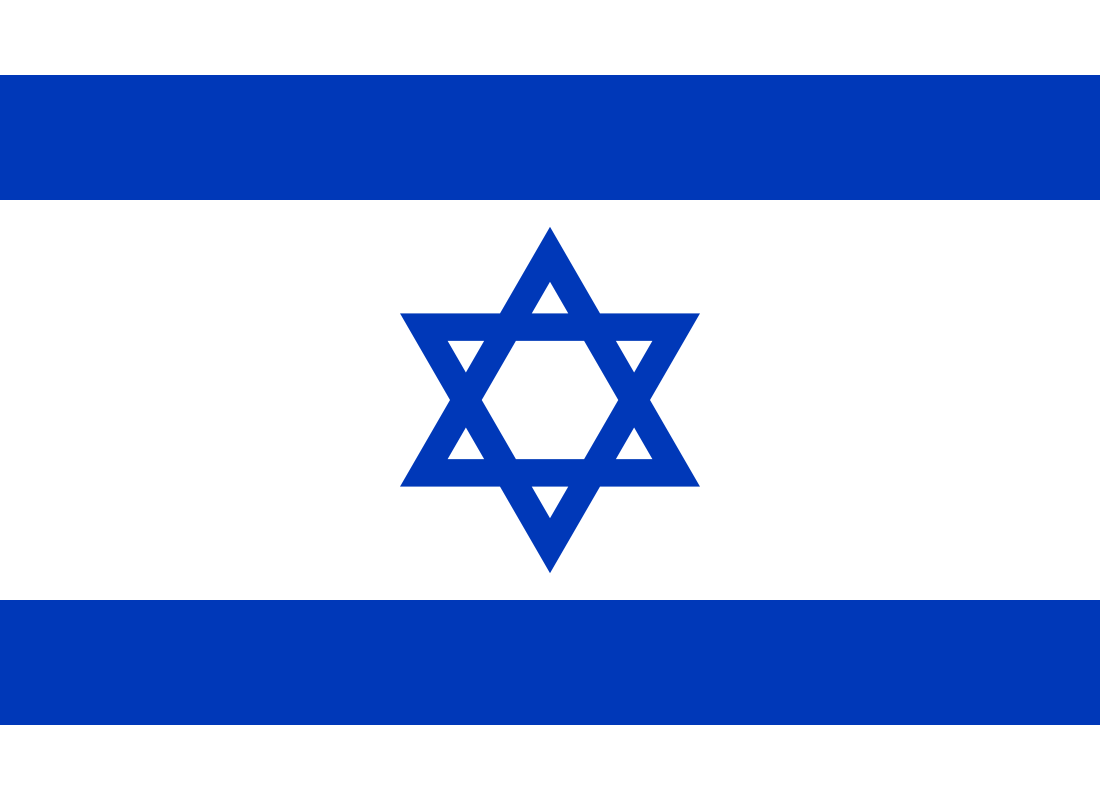
\includegraphics[width=\linewidth]{./chapter/country/256px-Flag_of_Israel.png}}%
	}
	\caption{Флаг третьей страны.}%
	\label{fig:flag_israel}%
\end{marginfigure}
\begin{marginfigure}[0.0cm]
	{
		\setlength{\fboxsep}{0pt}%
		\setlength{\fboxrule}{1pt}%
		\fcolorbox{gray}{gray}{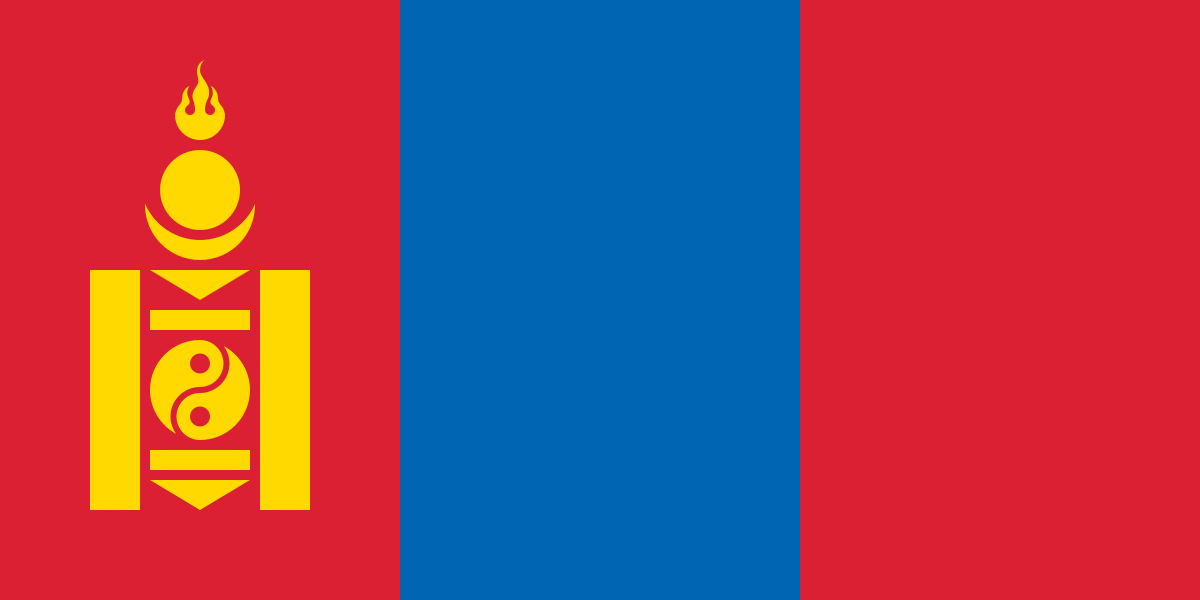
\includegraphics[width=\linewidth]{./chapter/country/256px-Flag_of_Mongolia.png}}%
	}
	\caption{Флаг четвертой страны.}%
	\label{fig:flag_mongolia}%
\end{marginfigure}
\marginnote{
	См. ответ~\ref{answer:population_density} на с.~\pageref{answer:population_density}.
}

\subsection{Страны с незаполненной датой основания}

Выведем список стран с пустым свойством <<дата основания>> (листинг ~\ref{lst:without_inception}).

\begin{lstlisting}[ language=SPARQL, 
caption={\href{https://w.wiki/k6q}{Страны с незаполненной датой основания}\protect\footnotemark},
label=lst:without_inception, 
escapebegin=ку,escapeend=ку-ку>
]
SELECT ?country ?countryLabel 
WHERE
{
		?country wdt:P31 wd:Q6256. # country
		
		MINUS { ?country wdt:P571 [] } . # inception of country is empty
		SERVICE wikibase:label { bd:serviceParam wikibase:language "en" }
}
\end{lstlisting}

\footnotetext{Получено  100 записей на 2017 год и 7 записей на 2020 год. Ссылка на SPARQL-запрос: \href{https://w.wiki/k6q}{https://w.wiki/k6q}}

%%%%%%%%%%%%%%%%%%%%%%%%%%%%%%%%%%%%%%%%%%%%%%%%%%%%%%%
\section{Этнохоронимы на русском языке}

Этнохороним — название жителей определённой местности, соотнесённое с топонимом. Например, Россия – россияне, россиянин, россиянка, Чехия – чехи, чех, чешка.

Помимо географического мотиватора, новых лексемы, используемые для определения происхождения либо принадлежности, происходят так же от этнических, политических, религиозных характеристик людей\cite{country_2}. 

Название жителей может определяться от наименования различных объектов земной поверхности — гор, островов, континентов. Так же обозначение места происхождения людей может зависеть от политико-административного делению. Например, для обозначения гражданства; Украина — украинцы, Канада - канадцы. Внутригосударственное деление также может породить новые наименования, Крым — крымчане.

Построим список стран, у которых есть этнохоронимы на русском языке.

Выведем список стран с пустым свойством <<дата основания>> (листинг ~\ref{lst:demonym}).

\begin{lstlisting}[ language=SPARQL, 
caption={\href{https://w.wiki/k72}{Этнохоронимы на русском языке}\protect\footnotemark},
label=lst:demonym, 
escapebegin=ку,escapeend=ку-ку>
]
SELECT ?country ?countryLabel 
WHERE
{
		?country wdt:P31 wd:Q6256.       # country
		?country wdt:P1549 ?demonym .    # has demonym
		FILTER((LANG(?demonym)) = "ru")
		SERVICE wikibase:label { bd:serviceParam wikibase:language "ru" }
}
GROUP BY ?country ?countryLabel
\end{lstlisting}

\footnotetext{Получено  28 записей на 2017 год и 99 записей на 2020 год. Ссылка на SPARQL-запрос: \href{https://w.wiki/k72}{https://w.wiki/k72}}


\subsection{Cписок этнохоронимов}

%%%%%%%%%%%%%%%% Упражнение 4 %%%%%%%%%%%%%%%%
\marginnote{
	Какие из этих языков являются официальными в \href{https://w.wiki/myt}{России}.
	\begin{itemize}
		\item \href{https://w.wiki/myv}{абазинский};
		\item \href{https://w.wiki/myx}{мокшанский};
		\item \href{https://w.wiki/myy}{эрзянский};
		\item \href{https://w.wiki/myz}{белорусский}.
	\end{itemize}
	См. ответ~\ref{answer:official_language} на с.~\pageref{answer:official_language}.
}

Выведем список всех этнохоронимом на русском языке (листинг ~\ref{lst:list_demonym}).

\begin{lstlisting}[ language=SPARQL, 
caption={\href{https://w.wiki/k7A}{Cписок этнохоронимов}\protect\footnotemark},
label=lst:list_demonym, 
escapebegin=ку,escapeend=ку-ку>
]
SELECT ?country ?countryLabel ?demonym
WHERE
{
		?country wdt:P31 wd:Q6256.      # country
		?country wdt:P1549 ?demonym.   # demonym
		FILTER((LANG(?demonym)) = "ru")
		SERVICE wikibase:label { bd:serviceParam wikibase:language "ru" }
}
\end{lstlisting}

\footnotetext{Получено  83 записи на 2017 год и 222 записи на 2020 год. Ссылка на SPARQL-запрос: \href{https://w.wiki/k7A}{https://w.wiki/k7A}}

\subsection{Страны с незаполненными этнохоронимами}

Построим список стран, у которых нет этнохоронимов на русском языке (листинг ~\ref{lst:without_demonym}).

\begin{lstlisting}[ language=SPARQL, 
caption={\href{https://w.wiki/k7E}{Страны с незаполненными этнохоронимами }\protect\footnotemark},
label=lst:without_demonym, 
escapebegin=ку,escapeend=ку-ку>
]
SELECT ?country ?countryLabel 
WHERE
{
		?country wdt:P31 wd:Q6256.              # country
		MINUS { ?country wdt:P1549 ?demonym.    # except with demonyms
			FILTER((LANG(?demonym)) = "ru") # in Russian
		}    
		SERVICE wikibase:label { bd:serviceParam wikibase:language "ru" }
}
GROUP BY ?country ?countryLabel
\end{lstlisting}

\footnotetext{Получено  170 записей на 2017 год и 83 записи на 2020 год. Ссылка на SPARQL-запрос: \href{https://w.wiki/k7E}{https://w.wiki/k7E}}

\subsection{Количество заполненных этнохоронимов у стран}

Выведем список стран, упорядоченный по количеству заполненных в Викиданных этнохоронимов (листинг ~\ref{lst:count_demonym}).

\begin{lstlisting}[ language=SPARQL, 
caption={\href{https://w.wiki/k7K}{Количество заполненных этнохоронимов у стран}\protect\footnotemark},
label=lst:count_demonym, 
escapebegin=ку,escapeend=ку-ку>
]
SELECT  ?country ?countryLabel (count(*) as ?count)
WHERE
{
		?country wdt:P31 wd:Q6256.      # country
		?country wdt:P1549 ?demonym.    # demonym
		SERVICE wikibase:label { bd:serviceParam wikibase:language "ru" }
}
GROUP BY ?country 
ORDER BY DESC(?count)
\end{lstlisting}

\footnotetext{Получено 199 записей на 2017 год и 167 записей на 2020 год. Ссылка на SPARQL-запрос: \href{https://w.wiki/k7K}{https://w.wiki/k7K}}

По данным на 2017 год наибольшее число этнохоронимов у Соединённых Штатов Америки (41 этнохороним), затем идут Великобритания (40), Германия (40) и Канада (36). А на 2020 год наибольшее число этнохоронимов у Германии (64 этнохоронима), Канады (60), США (60) и Польши (54).
%%%%%%%%%%%%%%%%%%%%%%%%%%%%%%%%%%%%%%%%%%%%%%%%%%%%%%%
\section{Формы правления стран}

Построим пузырьковую диаграмму форм правления стран (листинг ~\ref{lst:form_of_government}).

\begin{lstlisting}[ language=SPARQL, 
caption={\href{https://w.wiki/k7M}{Формы правления стран}\protect\footnotemark},
label=lst:form_of_government, 
escapebegin=ку,escapeend=ку-ку>
]
SELECT ?bfog ?form (count(*) as ?count)
WHERE 
{
	?country wdt:P31 wd:Q6256. # country
	?country wdt:P122 ?bfog. # subject's government
	OPTIONAL {
		?bfog rdfs:label ?form
		filter (lang(?form) = "ru")
	}
}
GROUP BY ?bfog ?form
ORDER BY DESC(?count) ASC(?form)
\end{lstlisting}

\footnotetext{Получено 30 записей на 2017 год и 29 записей на 2020 год. Ссылка на SPARQL-запрос: \href{https://w.wiki/k7M}{https://w.wiki/k7M}}

В результате выполнения запроса мы получаем пузырьковую диаграмму с наиболее распространенными формами правления в странах по 2017 году на рис. ~\ref{fig:bubble_chart_forms_of_government_countries_2017}, по 2020 году на рис.~\ref{fig:bubble_chart_forms_of_government_countries_2020}.

\begin{figure}
	{
		\setlength{\fboxsep}{0pt}%
		\setlength{\fboxrule}{1pt}%
		\fcolorbox{gray}{gray}{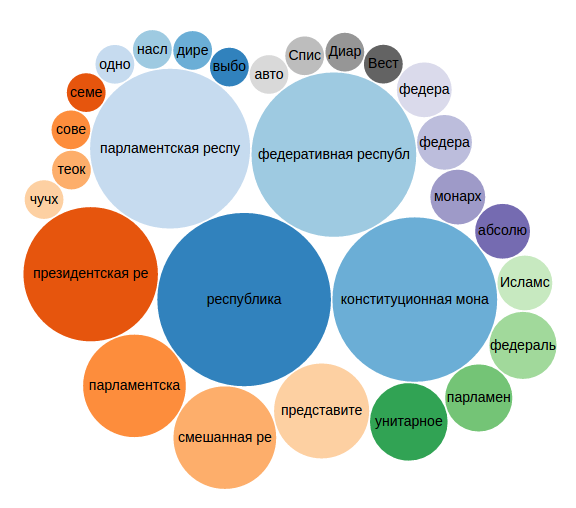
\includegraphics[width=\linewidth]{./chapter/country/Bubble_chart_forms_of_government_countries_according_to_Wikidata.png}}%
	}
	\caption{Пузырьковая диаграмма форм правления стран, 2017.
		\\			
		По данным на 2017 год основные формы правления стран: республика (в 20 странах), конституционная монархия (в 18 странах), федеративная республика (в 18 странах), парламентская республика (в 17 странах) и президентская республика (в 12 странах).}%
	\label{fig:bubble_chart_forms_of_government_countries_2017}%
\end{figure}

\begin{figure}
	{
		\setlength{\fboxsep}{0pt}%
		\setlength{\fboxrule}{1pt}%
		\fcolorbox{gray}{gray}{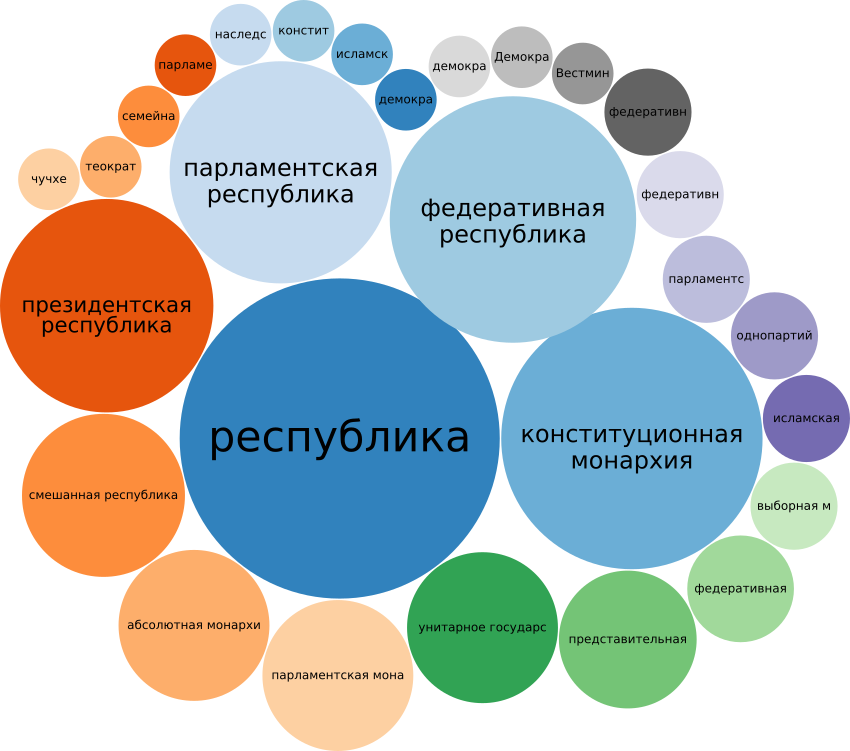
\includegraphics[width=\linewidth]{./chapter/country/Bubble_chart_forms_of_government_countries_according_to_Wikidata_2020.png}}%
	}
	\caption{Пузырьковая диаграмма форм правления стран, 2020.
	\\
	По данным на 2020 год  основные формы правления стран: республика (в 27 странах), конституционная монархия (в 18 странах), федеративная республика (в 16 странах), парламентская республика (в 13 странах) и президентская республика (в 12 странах).
}%
	\label{fig:bubble_chart_forms_of_government_countries_2020}%
\end{figure}

%%%%%%%%%%%%%%%%%%%%%%%%%%%%%%%%%%%%%%%%%%%%%%%%%%%%%%%
\section{Соседние страны}

Построим граф соседних стран (листинг ~\ref{lst:neighboring_countries}).

\begin{lstlisting}[ language=SPARQL, 
caption={\href{https://w.wiki/k7P}{Соседние страны}\protect\footnotemark},
label=lst:neighboring_countries, 
escapebegin=ку,escapeend=ку-ку>
]
SELECT ?country ?countryLabel ?sharesBorderWith ?sharesBorderWithLabel
WHERE
{
		?country wdt:P31 wd:Q6256.	# country
		SERVICE wikibase:label { bd:serviceParam wikibase:language "ru" }
		OPTIONAL { ?country wdt:P47 ?sharesBorderWith . }
}
\end{lstlisting}

\footnotetext{Получено имеет 787 записей на 2017 год и 698 записей на 2020 год. Ссылка на SPARQL-запрос: \href{https://w.wiki/k7P}{https://w.wiki/k7P}}

В результате выполнения запроса мы получаем граф с 787 ребрами на 2017 год (рис. ~\ref{fig:neighboring_countries_2017}) и 698 ребрами на 2020 год (рис. ~\ref{fig:neighboring_countries_2020}), где ребро – это соседство между двумя странами. Граф представляет из себя несколько связных компонент, так как есть островные страны, у которых нет соседей (например, Маврикий, Мальдивы, Мадагаскар).

\begin{figure}
	{
		\setlength{\fboxsep}{0pt}%
		\setlength{\fboxrule}{1pt}%
		\fcolorbox{gray}{gray}{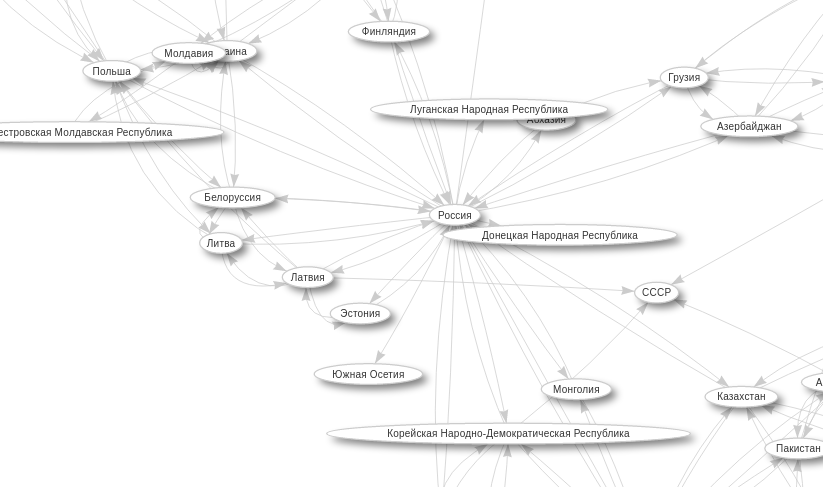
\includegraphics[width=\linewidth]{./chapter/country/Neighboring_countries_graph_in_russian_according_to_Wikidata_2017.png}}%
	}
	\caption{Фрагмент графа соседних стран, в центре Россия, 2017.
	}%
	\label{fig:neighboring_countries_2017}%
\end{figure}

\begin{figure}
	{
		\setlength{\fboxsep}{0pt}%
		\setlength{\fboxrule}{1pt}%
		\fcolorbox{gray}{gray}{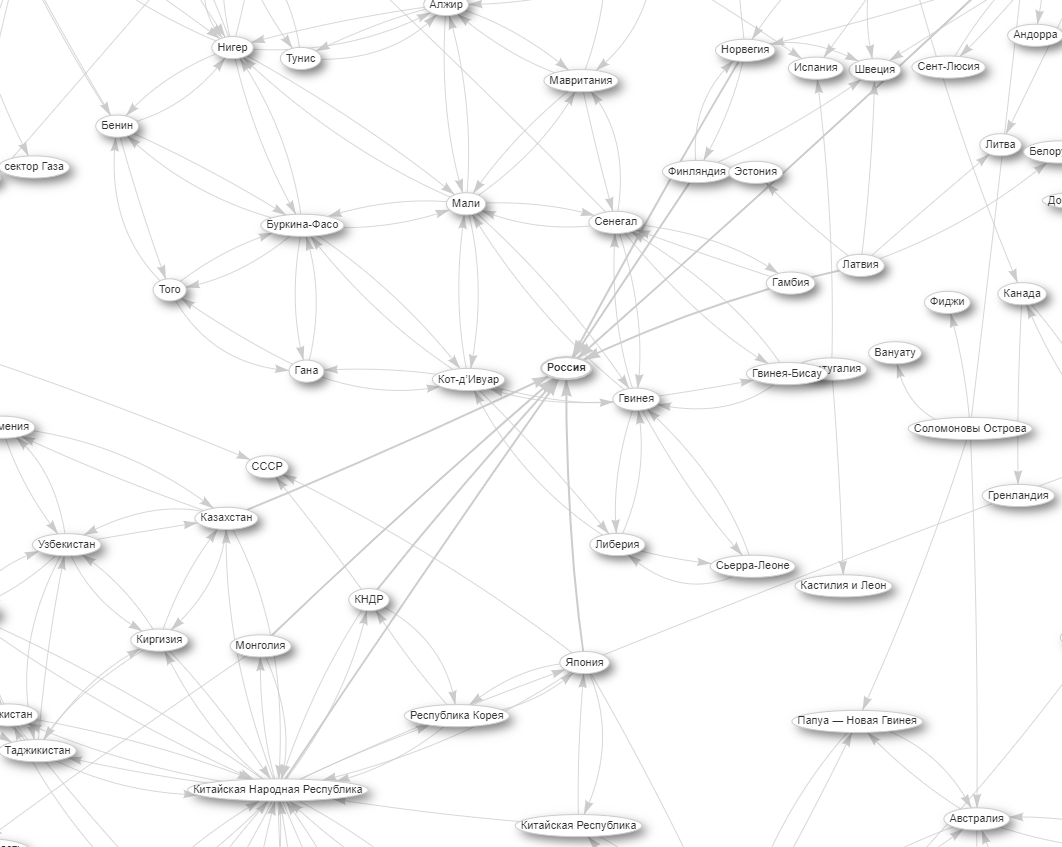
\includegraphics[width=\linewidth]{./chapter/country/Neighboring_countries_graph_in_russian_according_to_Wikidata_2020.png}}%
	}
	\caption{Фрагмент графа соседних стран, в центре Россия, 2020.
	}%
	\label{fig:neighboring_countries_2020}%
\end{figure}


%%%%%%%%%%%%%%%%%%%%%%%%%%%%%%%%%%%%%%%%%%%%%%%%%%%%%%%
\section{Упражнения}

\begin{enumerate}
	\item Постройте список флагов и девизов стран. Девизы есть не у всех стран.
	\item Отметьте на карте столицы современных стран.
	\item В каждой части света вычислите первые пять стран с наибольшей плотностью населения.
	\item Постройте столбчатую диаграмму, демонстрирующую распределение количества стран по формам правления. Оцените, является ли это распределение <<тяжелым хвостом>>.
	\item Выведите список стран упорядоченных по числу соседей. У каких стран максимальное и минимальное количество соседей, какое среднее число соседей? Есть ли корреляция между этим показателем и каким-либо другим параметром стран?
\end{enumerate}